\documentclass[dvipdfmx, twocolumn, a4paper]{hcresume}

\usepackage{epsfig}
\usepackage{amsmath}
\usepackage{graphics}
\usepackage{graphicx}
\usepackage{txfonts}
\usepackage{color}
\usepackage{BoldGothic4fig}
\usepackage{bm}
\usepackage{verbatim}
\usepackage{wrapfig}
\usepackage{ascmac}
\usepackage{makeidx}
\usepackage{enumerate}
\usepackage{comment}
\usepackage{multirow}
\usepackage{listings}
\usepackage{chngpage}

\usepackage[hang,small,bf]{caption}
\usepackage[subrefformat=parens]{subcaption}

%
\def\linesparpage#1{\baselineskip=\textheight
   \divide\baselineskip by #1}
\def\kcharparline#1{%
   \ifx\xkanjiskip\undefined%
   \jintercharskip 0mm plus 0.2mm minus 0.2mm
   \else
   \xkanjiskip 0mm plus 0.2mm minus 0.2mm
   \fi
   \settowidth{\textwidth}{}%
   \multiply\textwidth by #1}
%
\newcommand\figref[1]{\textbf{図~\ref{fig:#1}}}
\newcommand\tabref[1]{\textbf{表~\ref{tab:#1}}}
\newcommand{\bhline}[1]{\noalign{\hrule height #1}}

\hcheader{MIプログラム 卒業論文}
\title{\bf 評価者特性の時間変動を考慮した項目反応モデル}
\author{1810519 林真由}
\supervisor{指導教員 宇都 雅輝 准教授}

\begin{document}
\maketitle
\pagestyle{empty}
\thispagestyle{empty}
\section{はじめに}
近年,大学入試や資格試験,教育評価などにおいて,パフォーマンス評価のニーズが高まっている.一方で,パフォーマンス評価では,多肢選択式試験のような客観的評価と異なり人間の評価者が採点を行うため,評価者の厳しさや一貫性などの特性差がバイアス要因となり,受検者の能力測定の信頼性が低下する問題が知られている.このような問題を解決する数理的なアプローチの一つとして,評価者の特性を考慮した項目反応理論(Item response theory:IRT)\cite{IRTLord}が近年注目されている.

それらのIRTモデルを利用することで,評価者の特性差の影響を考慮した能力推定が可能となる.一方で,既存モデルのほとんどは評価者の特性が評価中に変化しないことを仮定している.しかし,多数の受検者を長時間かけて採点するような場合,
評価者の特性が採点の過程で変化する評価者ドリフト(Rater Drift)と呼ばれる現象がしばしば生じる.評価者ドリフトを考慮したモデルも提案されているが,既存モデルには評価者特性の時間変化を直線的にしか表現できないという問題点がある.

この問題を解決するために,本研究では,時間区分ごとの評価者の厳しさを推定できる新しいIRTモデルを提案する.
提案モデルでは,既存モデルよりも柔軟に評価者ドリフトを表現でき,モデルの性能が改善すると考えられる.本研究では,シミュレーション実験と実データ実験を通して提案モデルの有効性を示す.

\section{評価者特性を考慮した項目反応理論}
本研究では高精度な能力推定を行うためにIRTを利用する.

現在,評価者特性を最も柔軟に表現できるIRTモデルとして,一般化多相ラッシュモデルが知られている\cite{g-MFRM}.
このモデルでは,評価者$r$が受検者$j$のパフォーマンスにスコア$k$を与える確率を次式で定義する.
\begin{equation}
  P_{jrk}=\frac{\mathrm{exp}\sum_{m=1}^{k}\{\alpha_r(\theta_{j}-\beta_{r}-d_{rm})\}}{\sum_{l=1}^{K}\mathrm{exp}\sum_{m=1}^{l}\{\alpha_r(\theta_{j}-\beta_{r}-d_{rm})\}}
\end{equation}
ここで,$\alpha_r$は評価者$r$の一貫性,$\theta_j$は受検者$j$の能力,$\beta_r$は評価者$r$の厳しさ,$d_{rk}$は評価者$r$のスコア$k$に対する厳しさを表すステップパラメータである.モデルの識別性のために,$\sum^{K}_{k=2}{d_{rk}}=0$,$d_{r1}=0$を仮定する.

一般化多相ラッシュモデルは評価者の特性が評価中に変化しないことを仮定しているが,1章で述べたように,現実には評価者ドリフトという現象が起こる場合がある.
評価者ドリフトを考慮できるモデルとして,評価者$r$が時間区分$t$で採点した受検者$j$のパフォーマンスにスコア$k$を与える確率を次式で定義したモデルが提案されている.
\begin{equation}
  P_{jrtk}=\frac{\mathrm{exp}\sum_{m=1}^{k}(\theta_{j}-\beta_{r} - \pi_{r}t-d_{m})}{\sum_{l=1}^{K}\mathrm{exp}\sum_{m=1}^{l}(\theta_{j}-\beta_{r} - \pi_{r}t-d_{m})}
\end{equation}
ここで,$\beta_{r}$は評価者$r$の初期の厳しさ,$\pi_{r}$は評価者$r$の厳しさの変化の傾きを表す.

このモデルでは,一連の採点データを一定の時間区分に分割して作成したデータを用いる.具体的には,図\ref{timeid}のように,評価者が採点した順に受検者を並べ,データ全体をいくつかの時間区分数に分割し,インデックス(以降ではTimeIDと呼ぶ)を付与したデータである.

\begin{figure}[t]
  \centering
  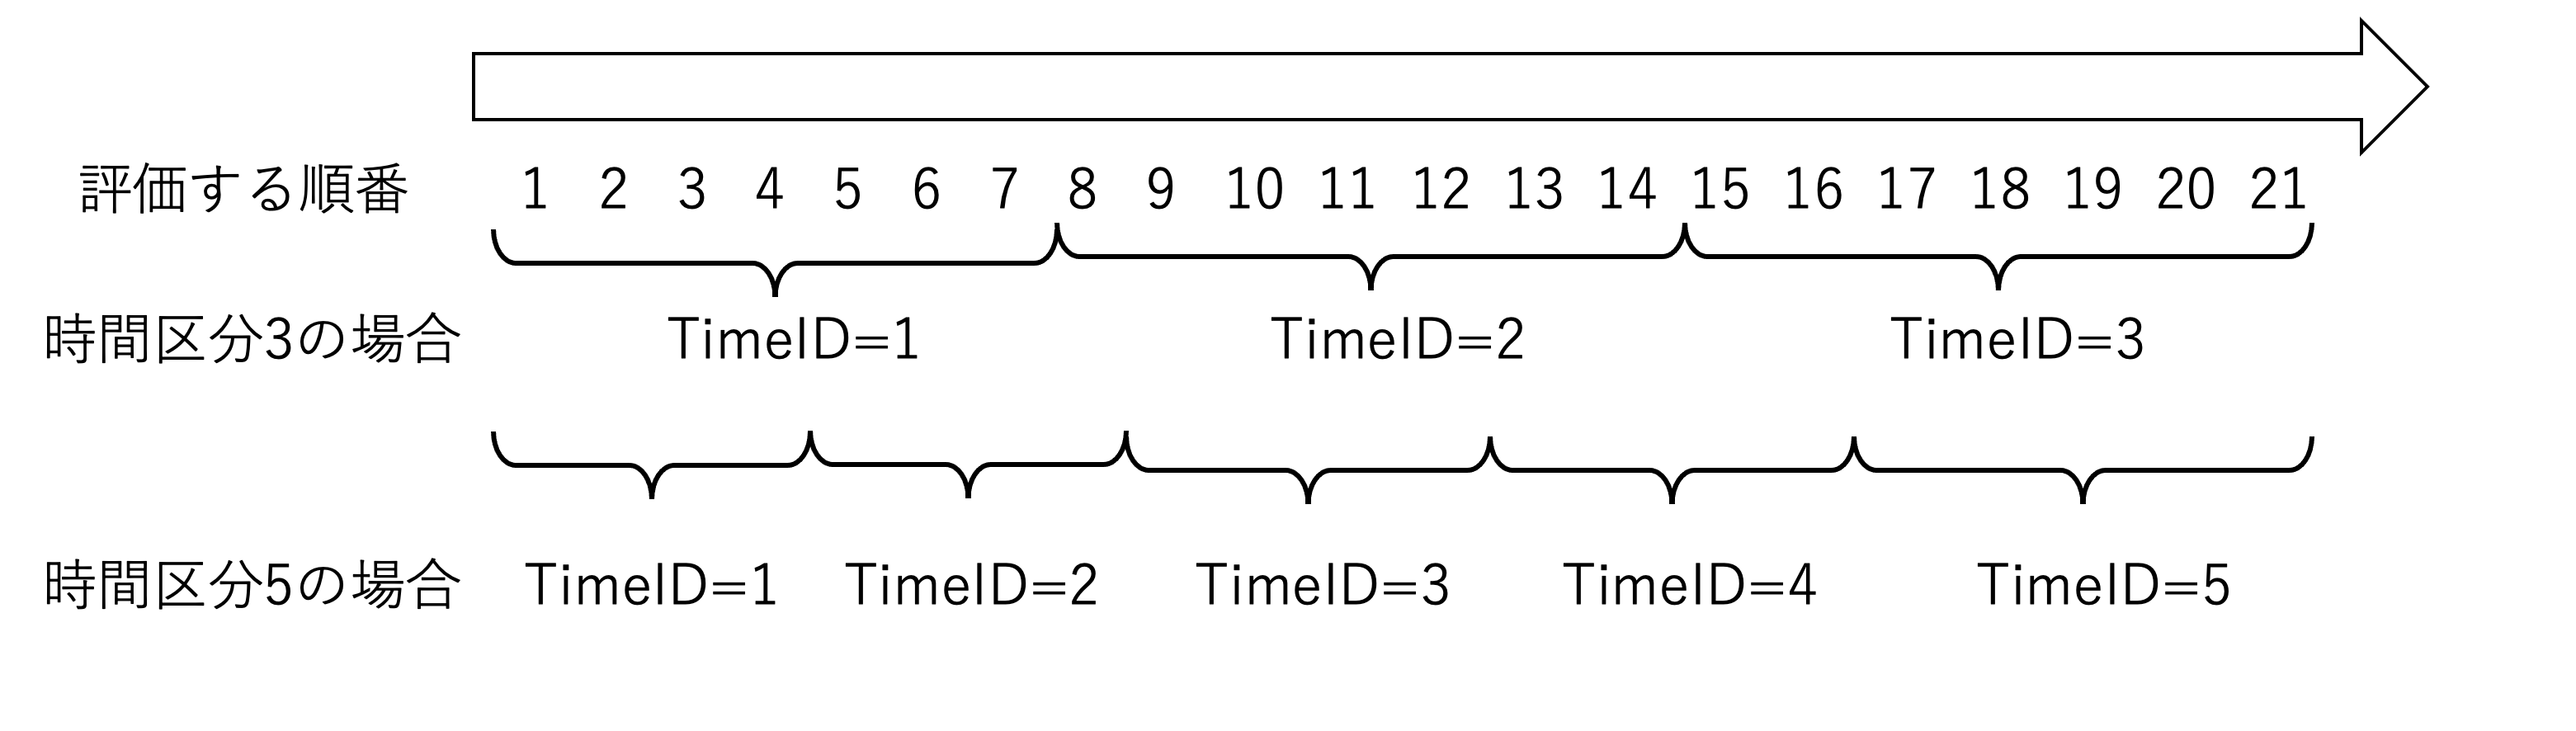
\includegraphics[width=8cm]{img/timeid.png}
  \caption{時間区分データのイメージと例}
  \label{timeid}
\end{figure}

このモデルでは時間経過による評価者特性の変化を捉えることができるが,その変化は直線的にしか表現できない.
この問題を解決するため,本研究では時間区分ごとの評価者の厳しさを推定できる新しいIRTモデルを提案する.
\section{提案モデル}
提案モデルでは,評価者$r$が時間区分$t$で採点した受検者$j$のパフォーマンスにスコア$k$を与える確率$P_{jrtk}$を次式で定義する.
\begin{equation}
  P_{jrtk}=\frac{\mathrm{exp}\sum^k_{m=1}{\alpha_r(\theta_{j}-\beta_{rt}-d_{rm})}}{\sum^K_{l=1} \mathrm{exp}\sum^l_{m=1}{\alpha_r(\theta_{j}-\beta_{rt}-d_{rm})}}
\end{equation}
\vspace{-5mm}
{\small
\begin{eqnarray}
  \beta_{rt}\sim \mathrm{N}(\beta_{r(t-1)},\sigma)\nonumber\\
  \beta_{r1} \sim \mathrm{N}(0,1)\nonumber\\
  \sigma \sim \mathrm{LN}(-3,0)\nonumber
\end{eqnarray}
}
ここで,$\beta_{rt}$は評価者$r$の時間区分$t$における厳しさである.また,$\mathrm{N}(\mu,\sigma^2)$は平均$\mu$,標準偏差$\sigma^2$の正規分布,$\mathrm{LN}(\mu,\sigma^2)$は平均$\mu$,標準偏差$\sigma^2$の対数正規分布を表す.

提案モデルでは,$\beta_{rt}$が$\beta_{(r-1)t}$に依存して決まると仮定している点が特徴である.また,提案モデルでは,より柔軟に評価特性を表現するために,一般化多相ラッシュモデルでも採用されている評価者の一貫性パラメータ$\alpha_r$と各スコアに対する厳しさパラメータ$d_{rk}$も導入している.

なお,$\beta_{rt}$は直前の時間区分の値から大きくは変動しないと考えられる.そこで,$\beta_{rt}$が従う分布の標準偏差$\sigma$が小さくなるように,ここでは,$\sigma$の事前分布に$\mathrm{LN}(−3,0)$を採用している.

また,提案モデルではモデルの識別性のために,$\theta_{j}\sim \mathrm{N}(0,1)$,$\prod_{r}\alpha_r=1$, $d_{r1}=0$, $\sum_{k=2}^{K}d_{rk}=0$を仮定する.

提案モデルのパラメータ推定手法にはマルコフ連鎖モンテカルロ法(Markov chain Monte Carlo methods:MCMC)を用いる.パラメータの事前分布は$\theta_{j}$, $d_{rk}$, $\mathrm{log}\alpha_{r}$, $\beta_{rt}\sim \mathrm{N}(0,1^{2})$とした.本研究では,MCMCのバーンイン期間は1000とし,1000$\sim$2000時点までの1000サンプルを用いる.
\section{シミュレーション実験}

本節では,MCMCによる提案モデルのパラメータ推定精度をシミュレーション実験により評価する.実験手順は以下の通りである.
(1)パラメータの真値を,前節に記載したパラメータの分布に従って生成する.
(2)手順(1)で生成したパラメータを用いて,提案モデルに従ってデータを生成する.
(3)手順(2)で生成したデータからMCMCを用いてパラメータ推定を行う.
(4)手順(3)で得られたパラメータ推定値と手順(1)で生成したパラメータ真値において,RMSE(Root Mean Square Error)とバイアスを求める.
(5)以上を5回繰り返し実行し,RMSEとバイアスの平均値を求める.

上記の実験を,受検者数$J=$60,90,120,評価者数$R=$10,15,時間区分数$T=$3,5,10の場合において行った.得点の段階数は$K=$5とした.
実験結果の一部を表\ref{parameters_recovery}に示す.

\begin{table}[t]
  \begin{minipage}[t]{8cm}
    \centering
    \caption{提案モデルのパラメータ・リカバリ実験の結果}
    \setlength{\tabcolsep}{5.pt}
    \scalebox{0.8}{
  \begin{tabular}{cccccccccccccc}  
  \bhline{1pt}
  \multirow{2}{*}{$J$} & \multirow{2}{*}{$R$} & \multirow{2}{*}{$T$}  && \multicolumn{4}{c}{RMSE} &&   \multicolumn{4}{c}{BIAS}  \\
  \cline{5-8}\cline{10-13}
    & & & & $\theta$ & $\alpha_r$ & $\beta_{rt}$ & $d_{rk}$ &  & $\theta$ & $\alpha_r$ & $\beta_{rt}$ & $d_{rk}$ \\
  \bhline{1pt}
  60 & 10 & 3  && 0.28 & 0.23 & 0.19 & 0.34 && -0.01 & 0.01 & -0.01 & 0.00 \\
     &    & 5  && 0.29 & 0.26 & 0.25 & 0.37 && 0.00  & 0.02 & -0.03 & 0.00 \\
     &    & 10 && 0.29 & 0.23 & 0.23 & 0.37 && 0.00  & 0.01 & 0.00  & 0.00 \\
  \cline{2-14}
     & 15 & 3  && 0.23 & 0.27 & 0.24 & 0.38 && 0.01  & 0.01 & 0.01  & 0.00 \\
     &    & 5  && 0.22 & 0.22 & 0.23 & 0.36 && 0.00  & 0.01 & 0.02  & 0.00 \\
     &    & 10 && 0.26 & 0.27 & 0.31 & 0.38 && -0.02 & 0.01 & -0.04 & 0.00 \\
   \hline
  120 & 10 & 3  && 0.26 & 0.19 & 0.15 & 0.27 && -0.01 & 0.01 & 0.00  & 0.00 \\
      &    & 5  && 0.28 & 0.21 & 0.18 & 0.32 && 0.00  & 0.01 & -0.01 & 0.00 \\
      &    & 10 && 0.28 & 0.20 & 0.25 & 0.29 && -0.01 & 0.00 & -0.03 & 0.00\\
  \cline{2-14}
  & 15 & 3  && 0.22 & 0.19 & 0.13 & 0.24 && 0.02 & 0.00 & 0.03 & 0.00 \\
  &    & 5  && 0.23 & 0.17 & 0.18 & 0.31 && 0.02 & 0.02 & 0.05 & 0.00 \\
  &    & 10 && 0.24 & 0.20 & 0.26 & 0.30 && 0.00 & 0.01 & 0.00 & 0.00 \\
  \hline
  \multicolumn{4}{c}{Avg.}   &  0.26 & 0.24 & 0.24 & 0.34 &  & 0.01 & 0.01 & 0.01 & 0.00 & \\
  \bhline{1pt}
  \end{tabular}
  }
    \label{parameters_recovery}
  \end{minipage}
\end{table}
  
表\ref{parameters_recovery}から,全パラメータのRMSEの平均値は$0.2\sim0.3$程度となり,十分に小さい値であると解釈できる.BIASについてもいずれのパラメータも0に非常に近い値を示しており,適切に推定できているといえる.また,関連研究(例:\cite{UtoUeno,YagiUto})と同様に,受検者数・評価者数の増加に伴い推定精度が改善する傾向が読み取れる.一方で,時間区分の総数Tが多くなると性能が低下する傾向も読み取れる.これはパラメータ数に対するデータ数が減少するためであり,合理的な傾向と考えられる.

以上の結果から, MCMCにより提案モデルのパラメータを適切に推定できることが確認できた.

\section{実データ実験}
本章では,実データの適用を通して,提案モデルの有効性を評価する.

本研究では,134名分のエッセイ課題を,16名の評価者が5段階得点で採点したデータを使用する.
評価者には,採点を4日に分け,日ごとに全体の1/4ずつ採点するように指示した.本実験では,これらの採点日ごとに時間区分1,2,3,4として扱う.なお,全16名の被験者のうち,6人には採点の際に指示を与え,人為的に評価者バイアスのあるデータを作成するようにした.

ここではまず,このように収集したデータに対して提案モデルを適用してパラメータを推定した.
$\beta_{rt}$の推定結果を図\ref{beta_rt_data}に示す.図では,縦軸が$\beta_{rt}$の値,横軸がTimeID,各線が一名の評価者の結果を表す.また例として,だんだん厳しくなるように指示した評価者の結果を赤色の線で示した.

図の赤線から,この評価者が想定通りに採点をしており,その特性を適切にモデルが捉えていることがわかる.指示をした他の評価者についても,指示通りの傾向が表現できていたことが確認できた.また,指示を与えていない評価者でも,評価者ドリフトが疑われる評価者が見受けられることがわかる.
以上から提案モデルが評価者ドリフトの傾向を推定できていることがわかる.

\begin{figure}[t]
  \centering
 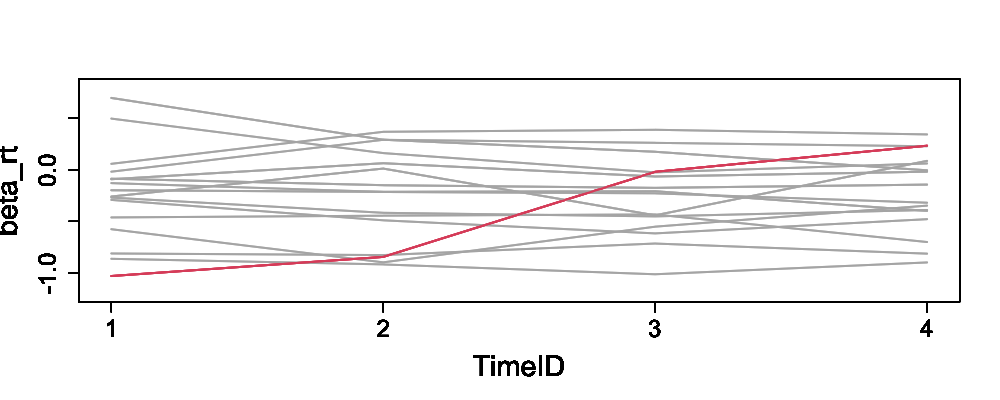
\includegraphics[width=8cm]{img/beta_rt_img_4.png}
 \caption{実データ実験による$\beta_{rt}$の推定結果}
 \vskip5mm
  \label{beta_rt_data}
\end{figure}
また,提案モデルの性能を評価するために,式(2)の既存モデルとの情報量規準によるモデル比較を行う.
加えて,既存モデルから提案モデルへのいくつかの変更点の中で,どの変更が効果を持っていたかを確認するために,以下の3つのモデルとの比較を行う.

\begin{description}
\item [比較モデル1]提案モデルの$d_{rk}$を$d_k$に入れ替え
\item [比較モデル2]提案モデルの$\beta_{rt}$を$\beta_{r} - \pi_{r}t$に置き換え
\item [比較モデル3]提案モデルの$\alpha_r$を削除
\end{description}

ここでは, MCMCにより各モデルのパラメータを推定し,得られた推定値を用いて情報量規準を求めた.情報量規準には
WAIC(Widely Applicable Information Criterion)とWBIC(Widely Applicable Bayesian Information Criterion)を用いた.どちらの基準も,値が小さい方が適したモデルであることを示す.

今回は,全ての評価者データを使用して推定を行った場合と,指示を与えた評価者を除外して推定を行った場合に分けて情報量基準を求めた.
表\ref{WAIC1}と\ref{WAIC2}から,WAICの最小値を比較すると,提案モデルが最適モデルとして選択されたことが確認できる.
また,この表から,提案モデルで追加した$\alpha_r$や$d_{rk}$を取り除くと性能が低下することも読み取れ,これらの有効性も確認できる.

次に,表\ref{WAIC1}と\ref{WAIC2}から,WBICの最小値を比較すると,比較モデル3と比較モデル1が最も高い性能を示しており,提案モデルより単純なモデルが最適なモデルとして選択されていることがわかる.一方で,提案モデルはどちらにおいても2番目に高い性能を示しており,$\beta_{rt}$にマルコフ性を導入したことの有効性は確認できる.

\begin{table}[tb]
  \centering
  % \begin{minipage}[]{9cm}
    \centering
    \caption{モデル比較の結果}
    \setlength{\tabcolsep}{1.pt}
    \scalebox{0.85}{
    \begin{tabular}{cccccc}  
      \bhline{1pt}
        &既存モデル&提案モデル&比較モデル1&比較モデル2&比較モデル3\\ 
        \cline{2-6}
        WAIC&5361.581&\textbf{5027.951}&5225.050&5104.463&5032.362\\
        \bhline{1pt}
        WBIC&3071.706&3033.753&3038.600&3056.349&\textbf{3028.649}\\
        \bhline{1pt}
      \end{tabular}
    }
    \label{WAIC1}
  % \end{minipage}
\end{table}
 
\begin{table}[tb]
  \centering
  % \begin{minipage}[]{9cm}
    \centering
    % \vskip5mm
    \caption{モデル比較の結果(指示なしの評価者)}
    \setlength{\tabcolsep}{1.pt}
    \scalebox{0.85}{
    \begin{tabular}{cccccccc}  
    \bhline{1pt}
     &既存モデル & 提案モデル & 比較モデル1 & 比較モデル2& 比較モデル3\\ 
     \cline{2-6}
    WAIC&3279.444 & \textbf{3134.700} & 3190.802 & 3154.331 & 3137.137\\
    \bhline{1pt}
      WBIC&1927.215 & 1900.211 & \textbf{1863.710} & 1924.210& 1910.699\\
      \bhline{1pt}
    \end{tabular}
    }
    \label{WAIC2}
  % \end{minipage}
\end{table}
\section{まとめと今後の課題}
本研究では,評価者の厳しさパラメータの時間変化を推定できる新しいIRTモデルを提案した.また,シミュレーション実験と実データを用いた実験を通して,提案モデルの有効性を示した.
今後の課題としては,今回提案したモデルは課題数1の場合を想定しており,課題ごとの特性を考慮することが出来ていない.そのため,課題パラメータを追加して課題ごとの特性を考慮したモデルを作ることが挙げられる.
{\small
\bibliographystyle{chukan}
\bibliography{chukan}
}
\end{document}